\documentclass{article}
\usepackage[a4paper, total={6in, 9in}]{geometry} % Set margins
\usepackage{graphicx} % Required for inserting images
\graphicspath{ {./images/} }
\usepackage[default,oldstyle,scale=1]{opensans} % Custom font
\usepackage[T1]{fontenc} % Custom font
\usepackage[]{xcolor, soul} % Custom colors
\usepackage[colorlinks = true,
            linkcolor = secondary,
            urlcolor = secondary,
            citecolor = secondary,
            anchorcolor = secondary] {hyperref} % Colored table of contents
\usepackage{titlesec} % Custom section titles 
\usepackage[most]{tcolorbox} % Visualize buttons in text
\usepackage{setspace} % adapt line spacing
\usepackage{wrapfig} % wrap text around images
\usepackage[font=small,labelfont=bf]{caption} % custom captions
\usepackage{subcaption} % captions for subfigures


% Custom commands
\newcommand{\term}[1]{\textcolor{secondary}{\textit{\textbf{#1}}}}
\newcommand{\button}[1]{{\tcbox{\textcolor{detail}{#1}}}}

% Custom colors
\definecolor{background}{rgb}{255, 255, 255}
\definecolor{primary}{RGB}{32, 30, 31}
\definecolor{secondary}{RGB}{189, 59, 74}
\definecolor{detail}{RGB}{248, 235, 236}
\definecolor{text1}{RGB}{102, 102, 102}
\definecolor{text2}{RGB}{51, 51, 51}

% Custom table of contents
\hypersetup{colorlinks=true, linkbordercolor=secondary,linkcolor=secondary}
\renewcommand{\contentsname}{\textcolor{secondary}{Innehållsförteckning}}

% Visualize buttons in text
\tcbset{on line, 
        boxsep=4pt, left=0pt,right=0pt,top=0pt,bottom=0pt,
        colframe=white,colback=secondary,  
        highlight math style={enhanced}
        }

\newcommand*{\img}[1]{%
    \raisebox{-.3\baselineskip}{%
        \includegraphics[
        height=\baselineskip,
        width=\baselineskip,
        keepaspectratio,
        ]{#1}%
    }%
}

% Screens
\fboxsep=2mm%padding thickness
\fboxrule=0.8pt%border thickness

% Adapt line spacing
\setstretch{1.50}

% Custom figure caption
\renewcommand{\figurename}{Figur.}

\def\title{Yotei}
\def\subtitle{Planeringsverktyg för Umeå Budoklubb}

\begin{document}
{

    \begin{titlepage}
        \begin{center}
            
\includegraphics[width=\textwidth]{images/ubk-logga.jpg}
            \break
            \huge\textbf{\title} \\
            \LARGE{{\subtitle}}\\
       \end{center}
    \end{titlepage}

    \newpage
       \tableofcontents
    \newpage
    

% Custom section titles
\titleformat{\section}
    {\normalfont\LARGE} % Font styling
    {\thesection} % Section number
    {1 em} % Space between number and title
    {}
    [{\color{secondary}\titlerule[0.8pt]}]

\titleformat{\subsection}[block]{\normalfont\Large\hspace{2em}}{\thesubsection}{1em}{}

\section{Introduktion}
    Detta är en användarhandledning för Umeå Budoklubbs planeringsverktyg, \textbf{Yotei}. Hemsidan är mobilanpassad och kan nås från alla enheter med internetuppkoppling. Yotei underlättar planeringsarbetet för tränare med sidor för att ge överblickar över grupper och deras tillfällen, listor för tekniker och övningar och en personlig sida som visar innehåll som du skapat, favoriserat samt dina kontoinställningar.

\section{Inloggning}
    \begin{wrapfigure}[10]{r}{0.31\textwidth}
        \vspace{-15pt}
        \fcolorbox{secondary}{background}{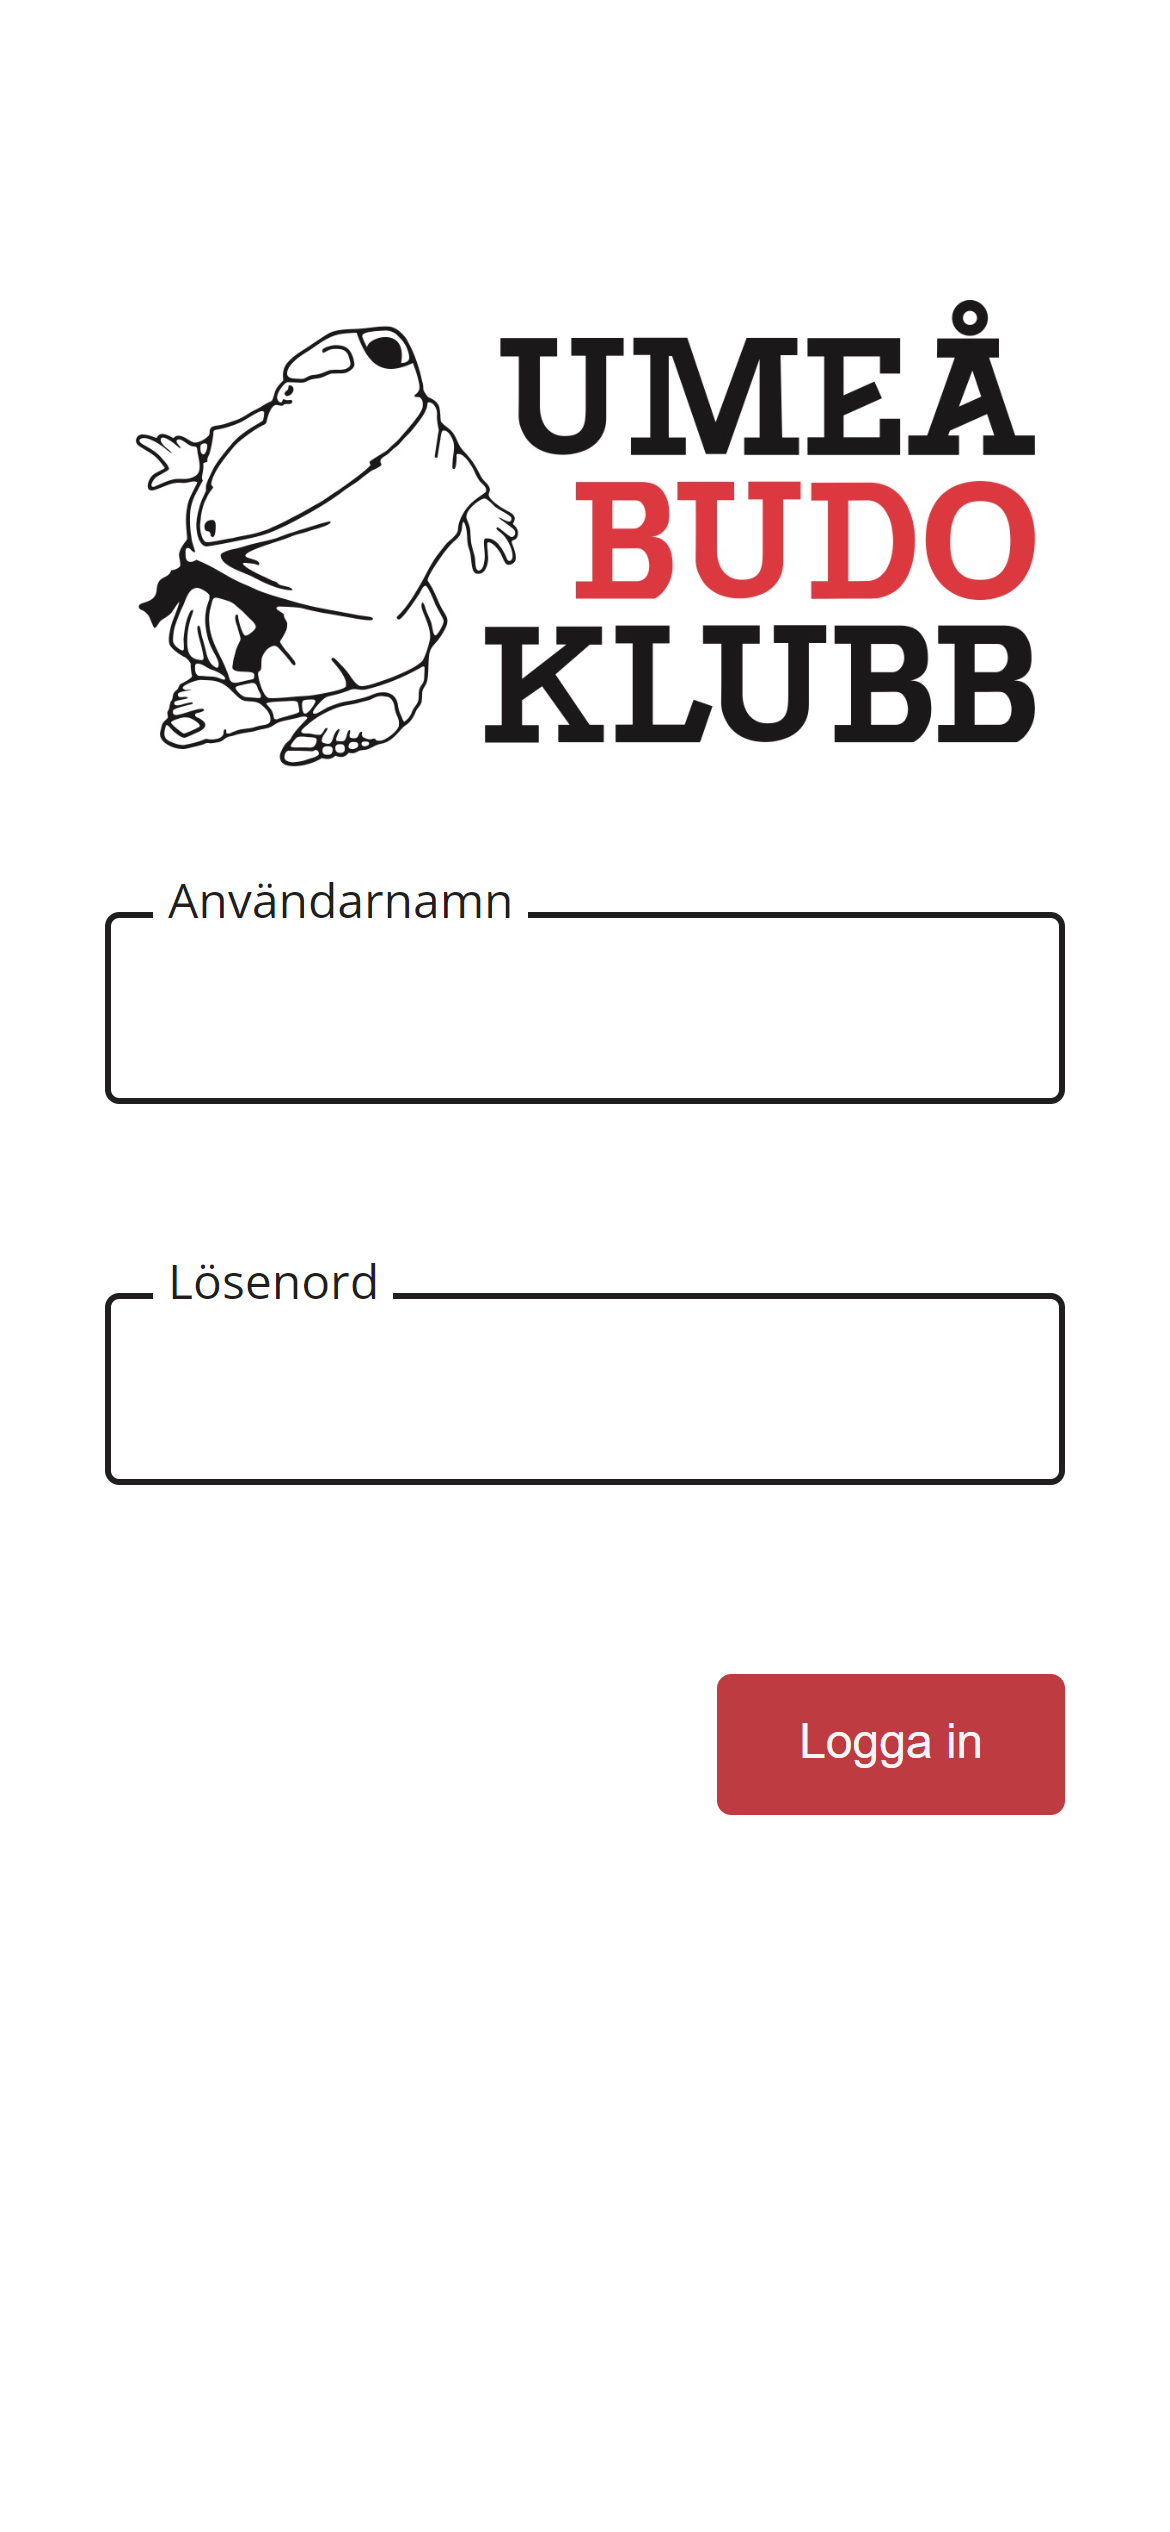
\includegraphics[width=0.9\linewidth]{images/Screens/Login.png}}
        \caption{Inloggningssidan.}
        \label{fig:login}
    \end{wrapfigure}
    När du går in på hemsidan möts du först av en sida som ber dig ange dina inloggningsuppgifter. Det är endast när du är inloggad som du kan nå de andra sidorna och ta del av innehållet. När du loggat in kommer du att komma till sidan där du kan se alla gruppers planeringar. För att logga in:
    \begin{enumerate}
        \item Skriv in ditt användarnamn, stor eller liten bokstav har ingen betydelse.
        \item Skriv in ditt lösenord, var noggrann med stor och liten bokstav samt nummer och specialtecken.
        \item Tryck på knappen \button{Logga in} eller \textit{Enter} på tangentbordet.
    \end{enumerate}
    \vspace{40pt}

\section{Navigation}
    \begin{wrapfigure}[5]{l}{0.25\textwidth}
        \vspace{-15pt}
        \fcolorbox{secondary}{background}{\includegraphics[width=0.9\linewidth]{images/Screens/NavBar.png}}
        \caption{Navigeringsmenyn som finns på alla sidor.}
        \label{fig:navbar}
    \end{wrapfigure}
    
    På varje sida \textit{(förutom inloggningssidan)} finns en navigationsmeny, du öppnar den genom att trycka på \img{images/icons ref/menu.png} längst upp i det vänstra hörnet. Här hittar du till snabblänkar till \term{Planering},\term{Grupper}, \term{Pass}, \term{Övningar}, \term{Tekniker} och \term{Min sida}. Om du är inloggad med en admin användare kan du även nå sidan \term{Admin} från navigationsmenyn.

\newpage
\section{Planering}
    På planeringssidan ser du alla gruppers tillfällen inom de kommande två åren. Tillfällena är grupperade efter veckor så att du enklare kan se när ett tillfälle tar plats. Du kan ändra hur många tillfällen som visas genom att trycka på filtreringsknappen \img{images/icons ref/Filter.png}. Där kan du ändra datumintervallet för tillfällena som ska visas eller vilka gruppers tillfällen som ska visas. Om du lämnar sidan kommer filteringen sparas så länge som du inte loggar ut. Ett tillfälle visar gruppens namn och bälten samt tillfällets datum, tid och dag. Om du trycker på ett tillfälle öppnas det och visar information om det finns pass som är kopplat. Om du vill lägga till ett nytt tillfälle för en grupp kan du trycka på plusknappen \img{images/icons ref/RoundButton.png} nere i det högra hörnet. Om du vill se alla grupper som finns trycker du på gruppknappen \img{images/icons ref/GroupButton.png}. 

    \begin{wrapfigure}[14]{R}{0.4\textwidth}
        \fcolorbox{secondary}{background}{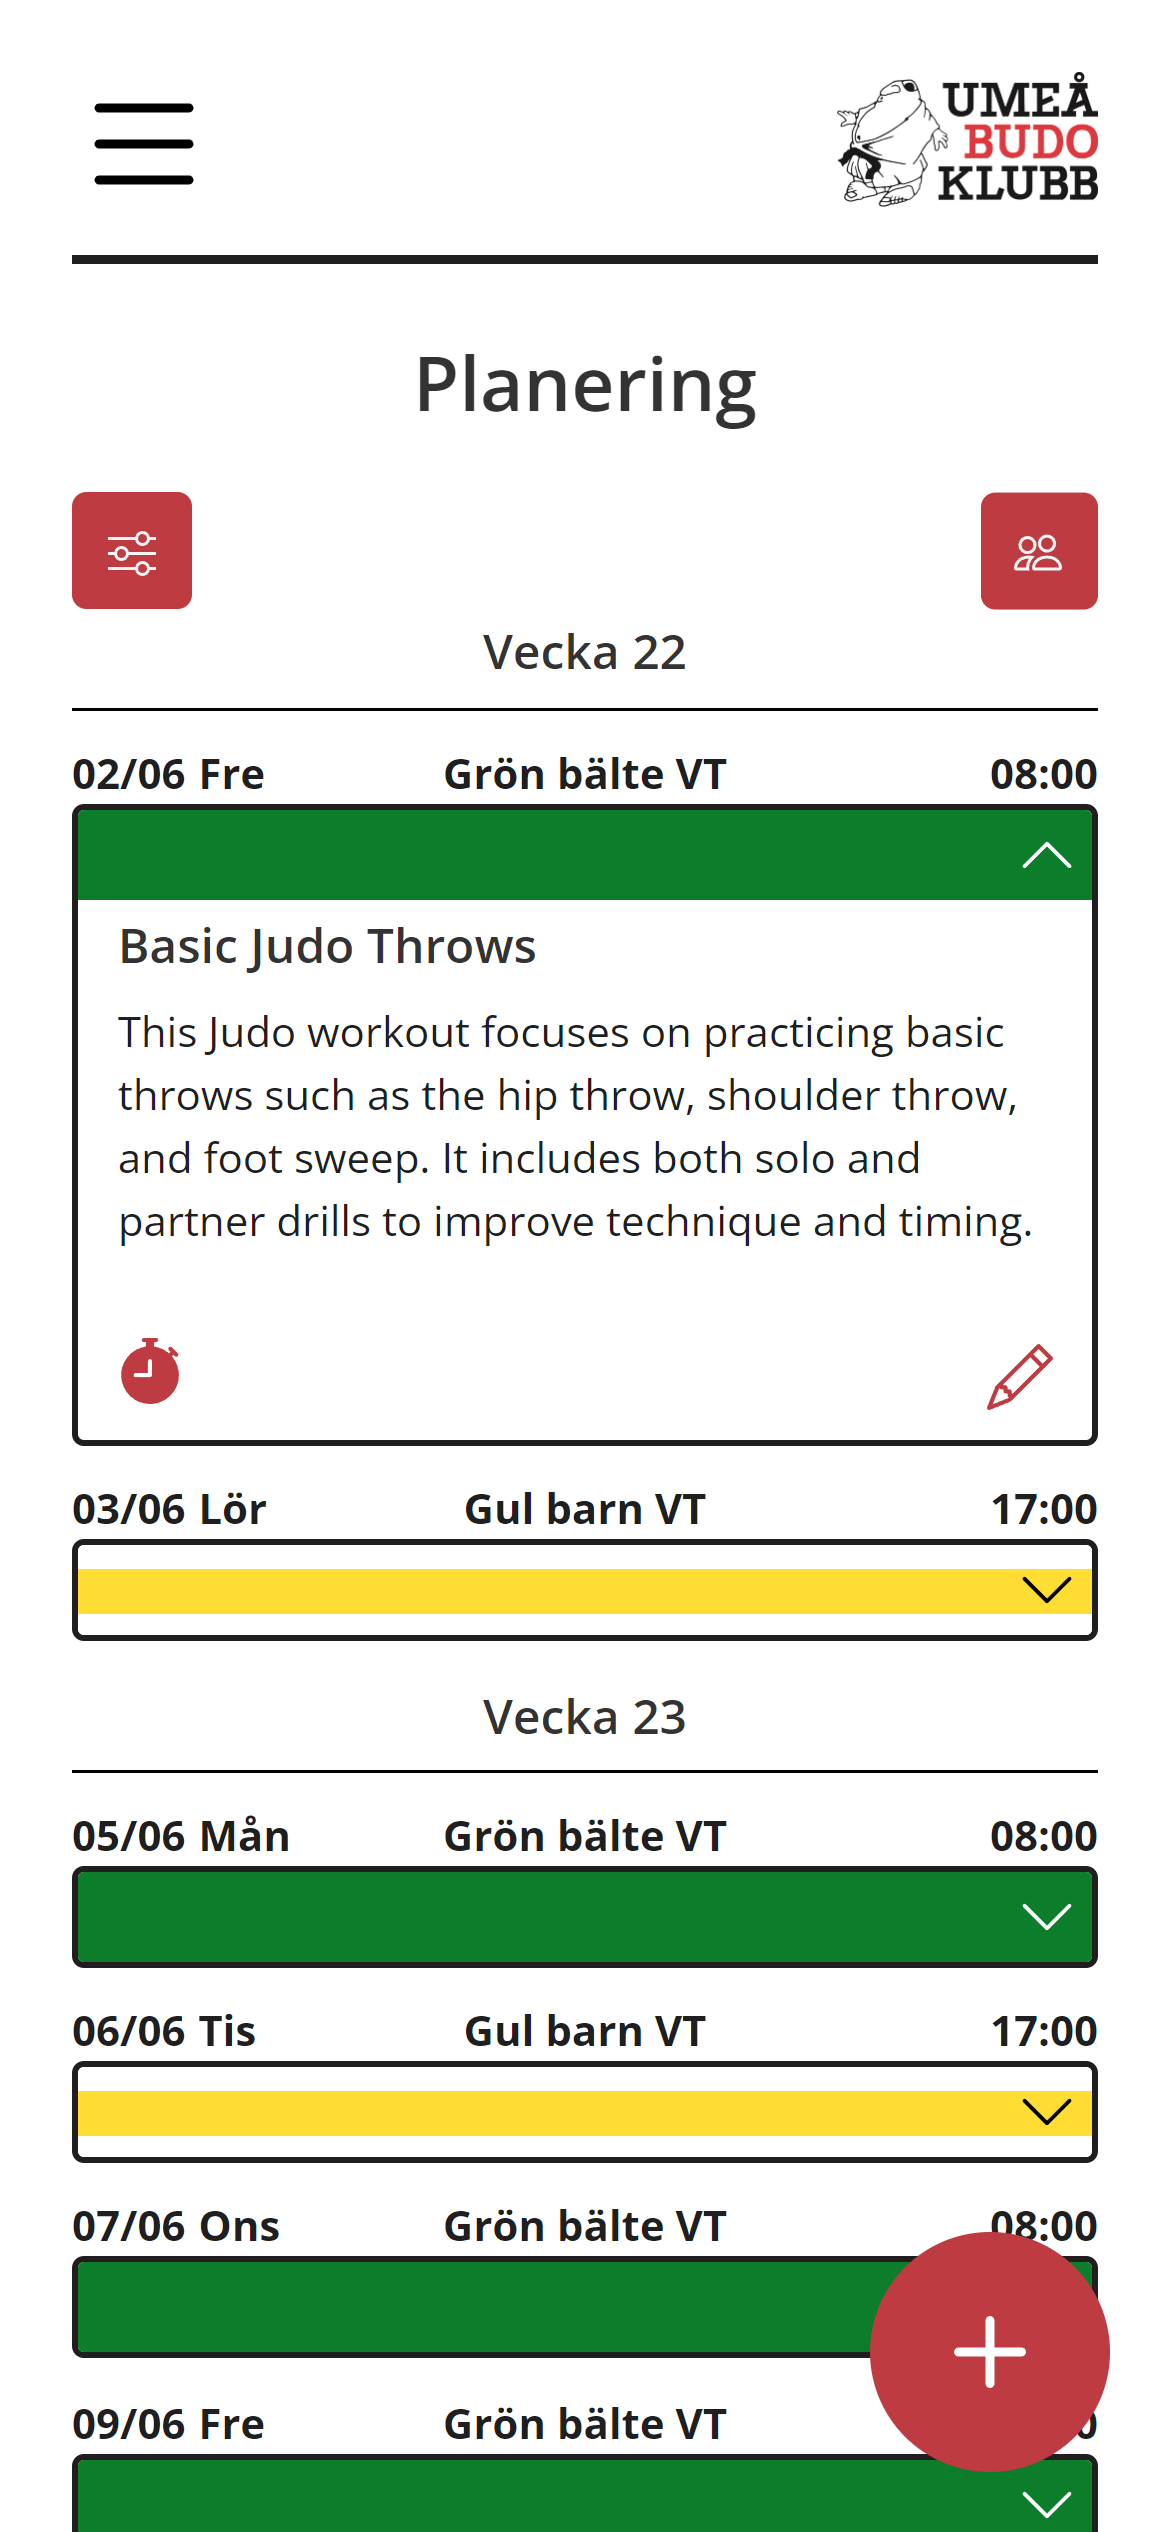
\includegraphics[width=0.9\linewidth]{images/Screens/GroupPlan.png}}
        \caption{Planeringssidan som innehåller olika gruppers tillfällen.}
        \label{fig:groupPlan}
    \end{wrapfigure}
    \subsection{Tillfällen}
        En grupp kan ha flera tillfällen och de skapas när du skapar en grupp och väljer att skapa återkommande tillfällen eller när du skapar ett enskilt tillfälle. Ett tillfälle kan ha ett pass kopplat till sig och det kan du koppla direkt när du skapar ett enskilt tillfälle eller när du redigerar ett som redan finns. Du kan redigera ett tillfälle genom att trycka på pennan \img{images/icons ref/pencil}, då kommer du till tillfällets redigeringssida. Det är bara du, en editor eller en admin som kan redigera dina egna tillfällen och grupper. Du kan se om ett tillfälle har ett pass eller inte genom att öppna det på planeringssidan. Om det finns ett pass kopplat kan du se namnet och beskrivningen på passet. Genom att klicka på stoppuret \img{images/icons ref/stopwatch.png} så kommer du till passets detaljsida. Om det inte finns ett pass så kan du koppla ett på redigeringssidan.

    \newpage
    \subsection{Grupper}
        \begin{wrapfigure}[14]{R}{0.4\textwidth}
            \vspace{-15pt}
            \fcolorbox{secondary}{background}{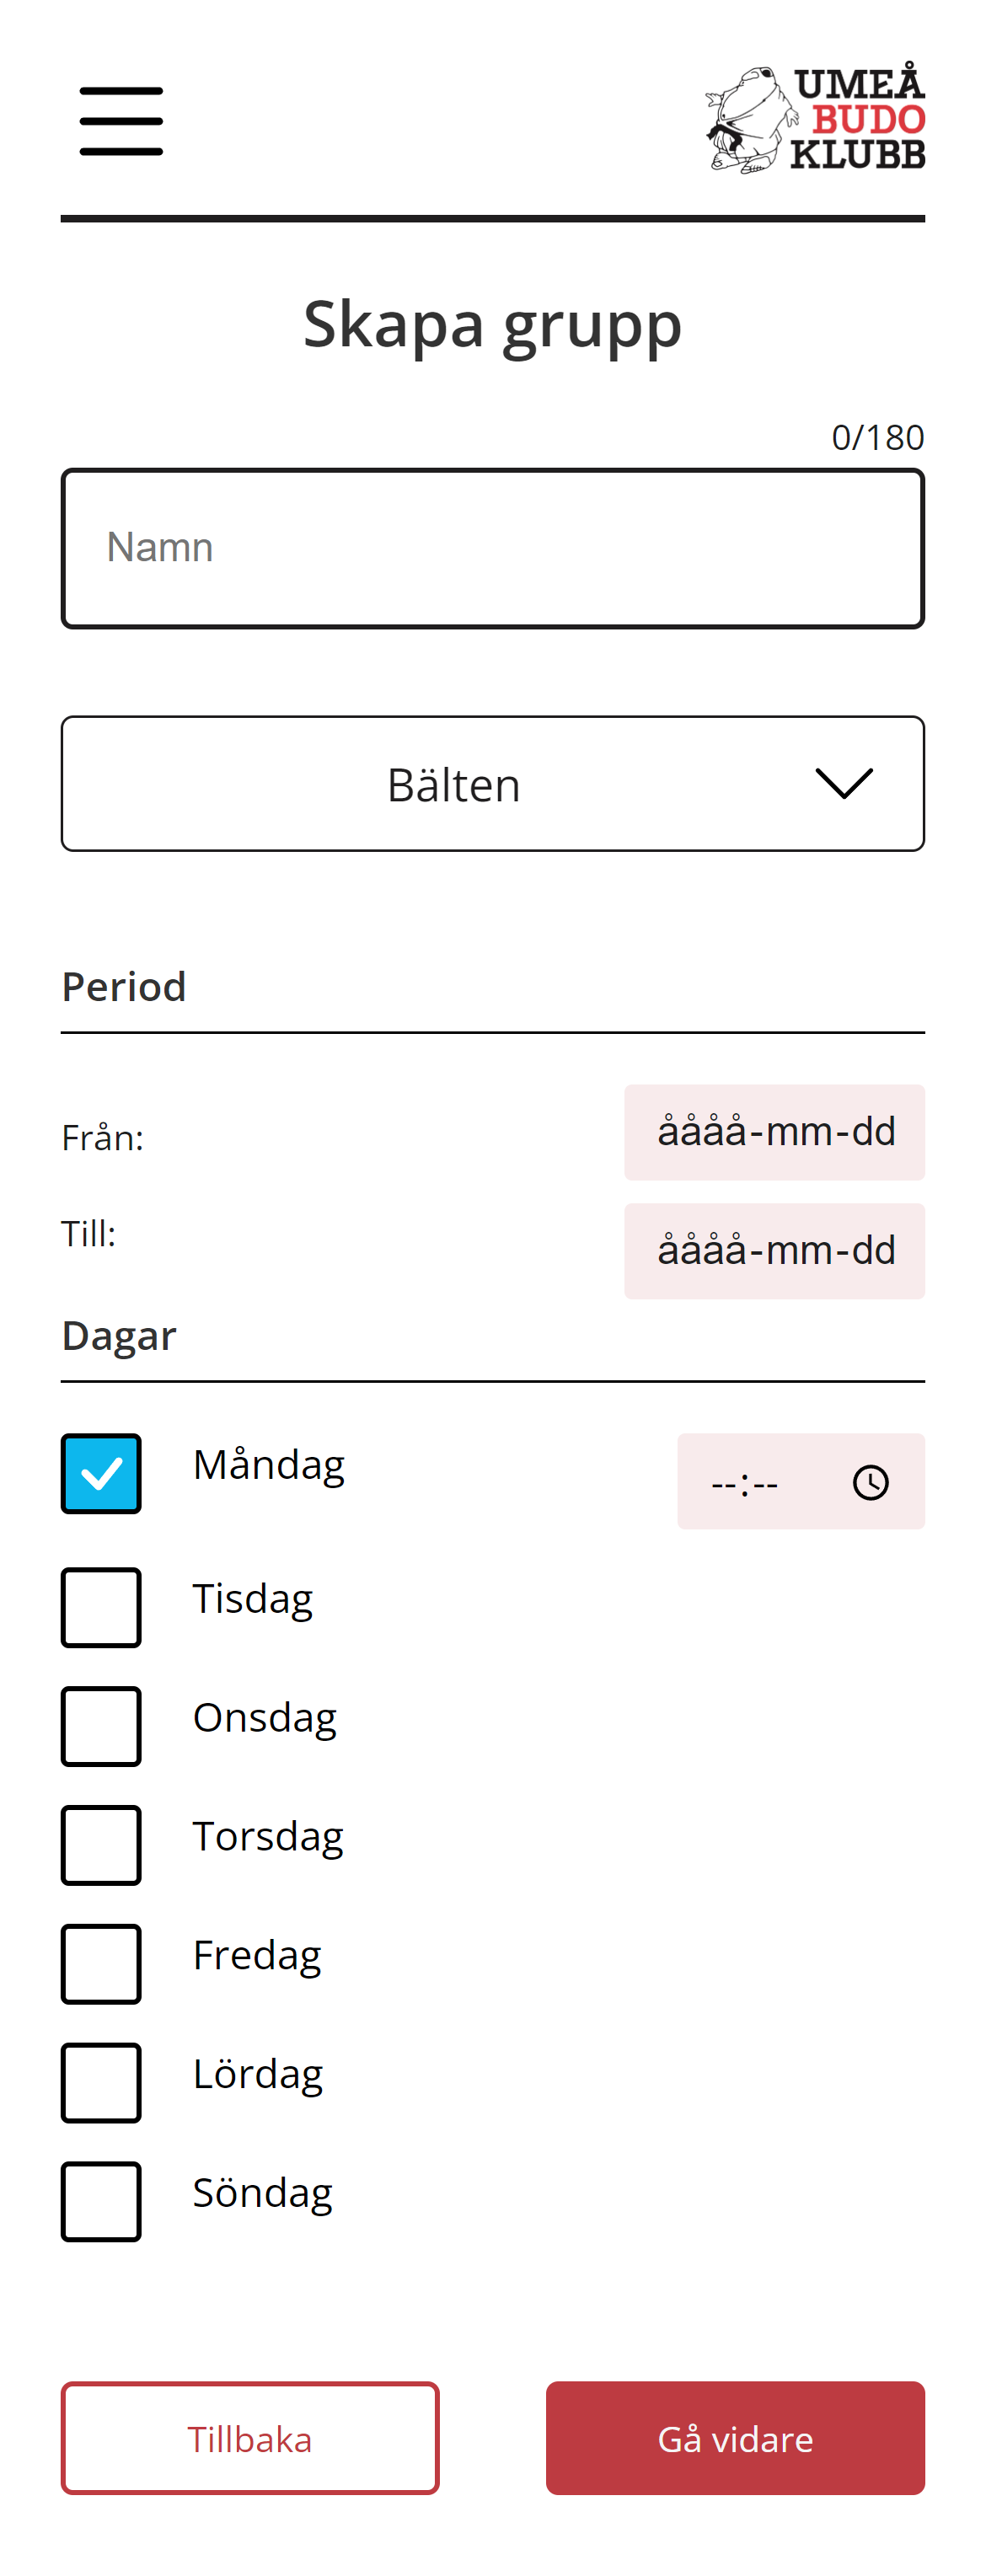
\includegraphics[width=0.9\linewidth]{images/Screens/GroupCreate.png}}
            \caption{Sidan för att skapa en ny grupp.}
            \label{fig:groupCreate}
        \end{wrapfigure}
        På gruppsidan ser du alla grupper som finns, både som du eller andra användare har skapat. Om du vill lägga till en ny grupp så trycker du på plusknappen \img{images/icons ref/RoundButton.png} nere i det högra hörnet. Där får man välja ett namn för gruppen, vilka bälten som ingår i gruppen, samt mellan vilka två datum som gruppens planering sträcker sig. Sedan får du välja på vilka dagar under denna planering som tillfällen ska skapas, och vilken tid. Exempelvis varje söndag klockan 17.00 under denna period. En grupp består alltså av en lista med tillfällen. Om du trycker på redigeringsknappen \img{images/icons ref/pencil.png} så kommer du till en sida där du kan redigera gruppen genom att ändra namn och bälten.
        
        \begin{figure}[h]
            \fcolorbox{secondary}{background}{
            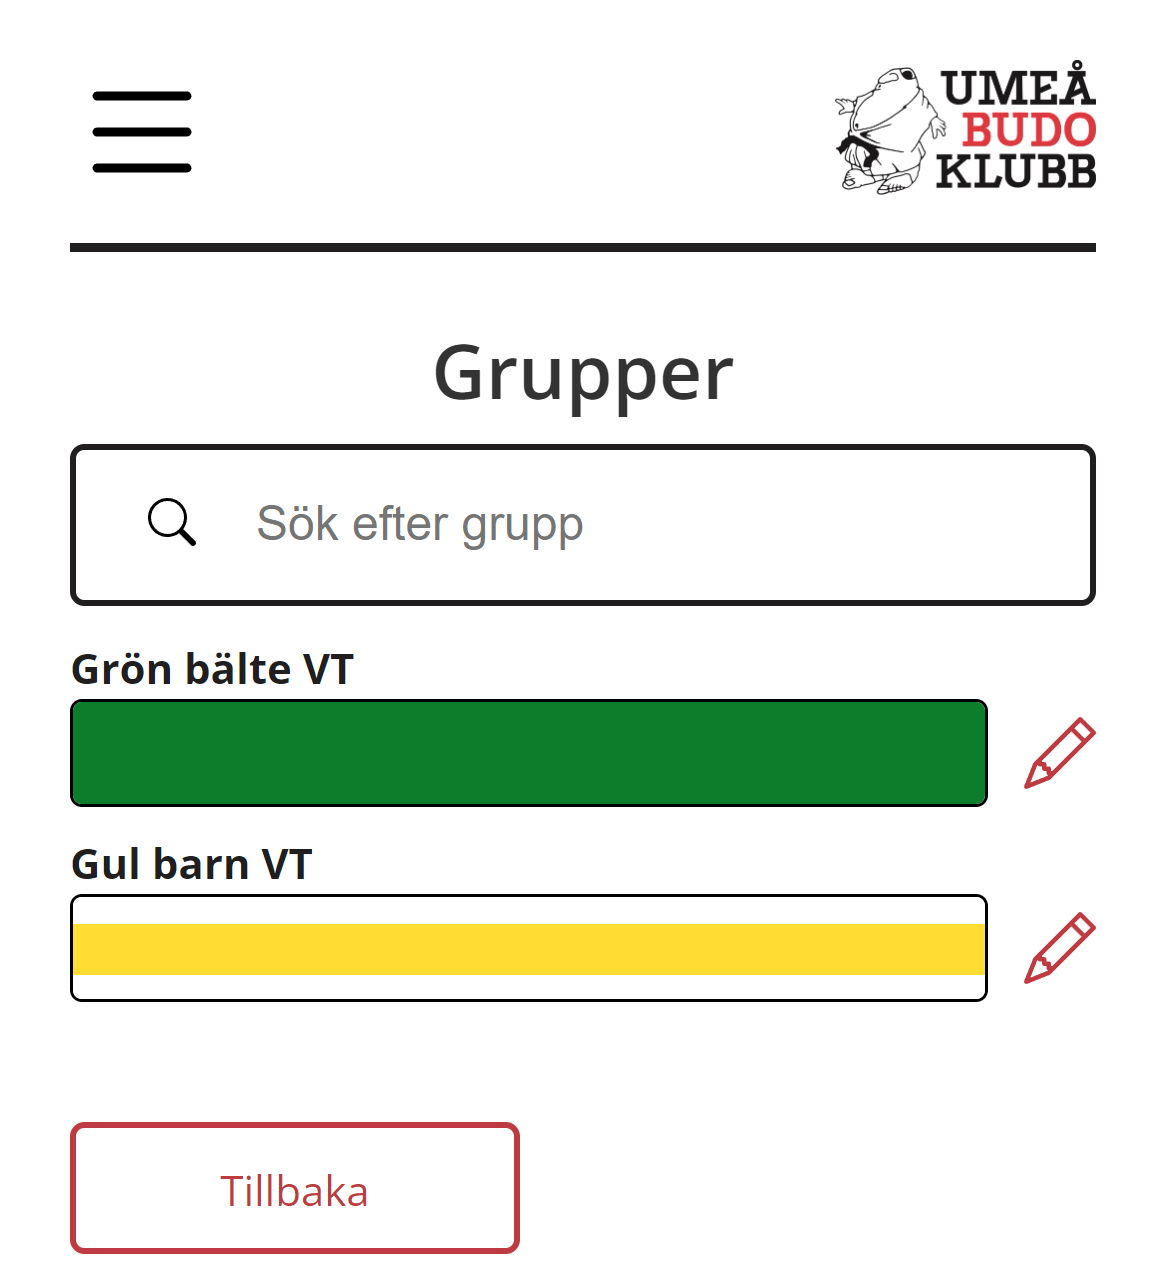
\includegraphics[width=0.3\textwidth]{images/Screens/Group.png}}
            \label{fig:groupFig}
        \end{figure}
        \noindent\textbf{Figur. 4.1:} Sidan för att visa grupper.\\
        \vspace{-5pt}
        \begin{figure}[h!]
            \fcolorbox{secondary}{background}{
            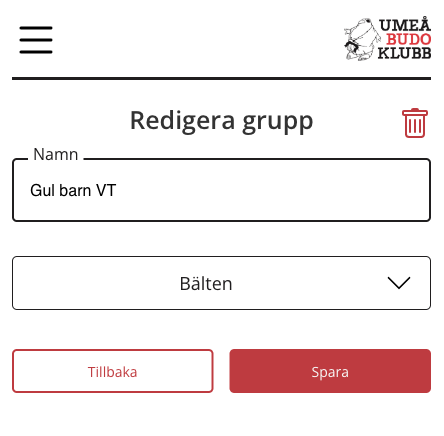
\includegraphics[width=0.3\textwidth]{images/Screens/GroupEdit.png}}
            \label{fig:groupFig}
        \end{figure}\\
        \textbf{Figur. 4.2:} Sidan för att redigera grupper.        

\newpage   
\section{Pass}
    \begin{wrapfigure}[14]{r}{0.3\textwidth}
        \vspace{15pt}
        \fcolorbox{secondary}{background}{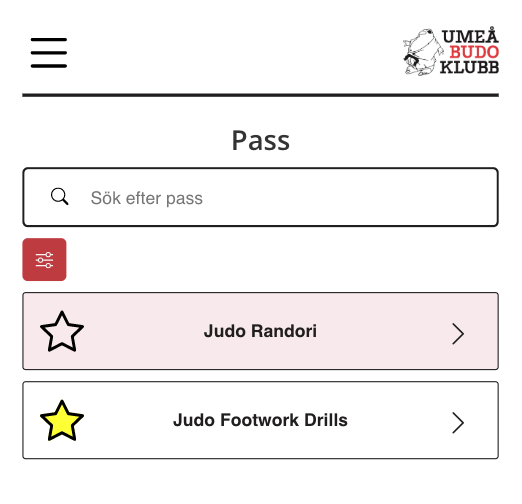
\includegraphics[width=0.9\linewidth]{images/Screens/Workout.png}}
        \caption{Passidan som visar alla pass.}
        \label{fig:workouts}
        \vspace{-40pt}
    \end{wrapfigure}
    På pass-sidan kan du se, ändra, ta bort och lägga till pass. Du kan söka bland passen som finns via sökrutan som du hittar under titeln för sidan. Du kan välja att söka antingen efter namnet på passet eller taggarna som passet har, till exempel \textit{Uppvärmning} eller \textit{Spark}. Du kan filtrera de pass som visas genom att trycka på \img{images/icons ref/Filter.png} och välja ett datumintervall. Datumintervallet baseras på när passet skapades. Du har även möjlighet att favorisera pass som du tycker mycket om. Det gör du genom att trycka på stjärnan \img{images/icons ref/star.png} bredvid passets namn. De pass som du favoriserat hittar du samlade på \term{Min sida}. Varje pass har en detaljsida där du kan se mer information om passet som passets beskrivning, vem som skapade det, när det skapades, när det senast ändrades och hur långt passet är. För att ta dig till denna sida trycker du på passet i listan med alla pass. På denna sida kan du även skriva ut ett pass.

    \begin{wrapfigure}[20]{r}{0.3\textwidth}
        \vspace{15pt}
        \fcolorbox{secondary}{background}{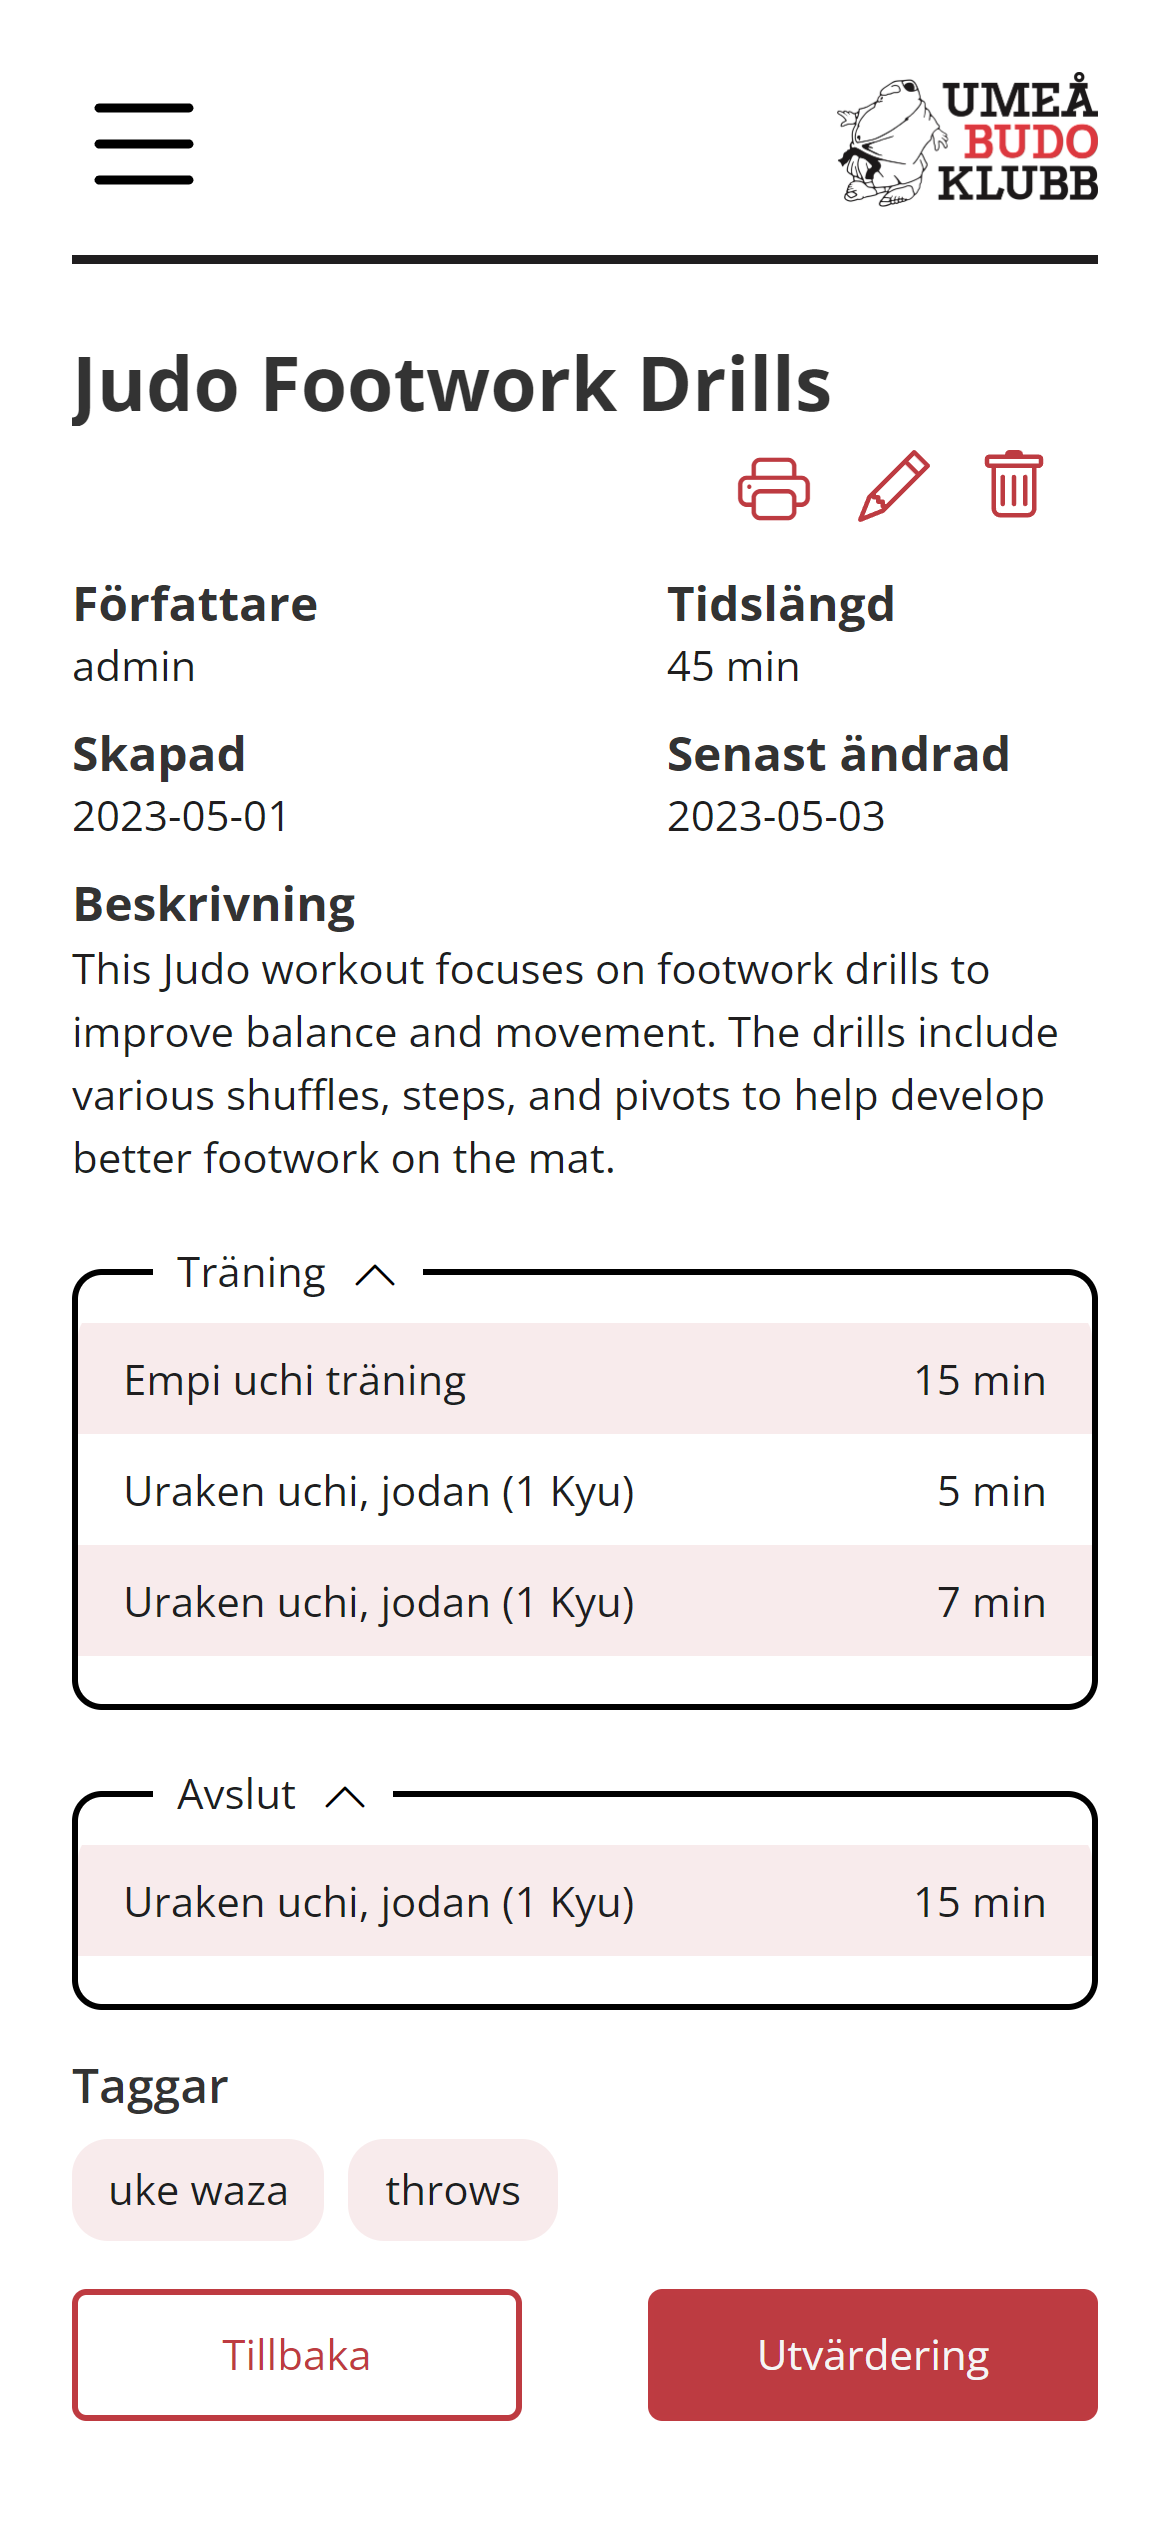
\includegraphics[width=0.9\linewidth]{images/Screens/WorkoutDetails.png}}
        \caption{Ett pass detaljsida.}
        \label{fig:workoutDetails}
    \end{wrapfigure}
    \subsection{Taggar}
        Ett pass kan ha noll, en eller flera taggar. Taggar används för att kategorisera passen och gör det möjligt att hitta de när man söker på taggarna i sökfunktionen. Du kan antingen söka bland redan existerande taggar eller skapa en ny. Taggar ignorerar små och stora bokstäver, det betyder att du kan inte lägga till taggen \textit{"blå"} om taggen \textit{"BLÅ"} redan finns. Man kan inte redigera eller ta bort taggar som blivit skapade.

    \subsection{Utvärdering}
        När passet är skapat går det att lägga till en utvärdering för passet. Det gör man genom att klicka på knappen \button{Utvärdering} längst ned på passets detaljsida. Alla som kan se passet kan skriva en utvärdering om det. I utvärderingen ingår en 5-skalig gradering av hur passet gick, en positiv kommentar och en kommentar om vad som var mer negativt med passet.

    \newpage
    \subsection{Lägga till pass}
        \begin{wrapfigure}[15]{r}{0.3\textwidth}
            \vspace{-15pt}
            \fcolorbox{secondary}{background}{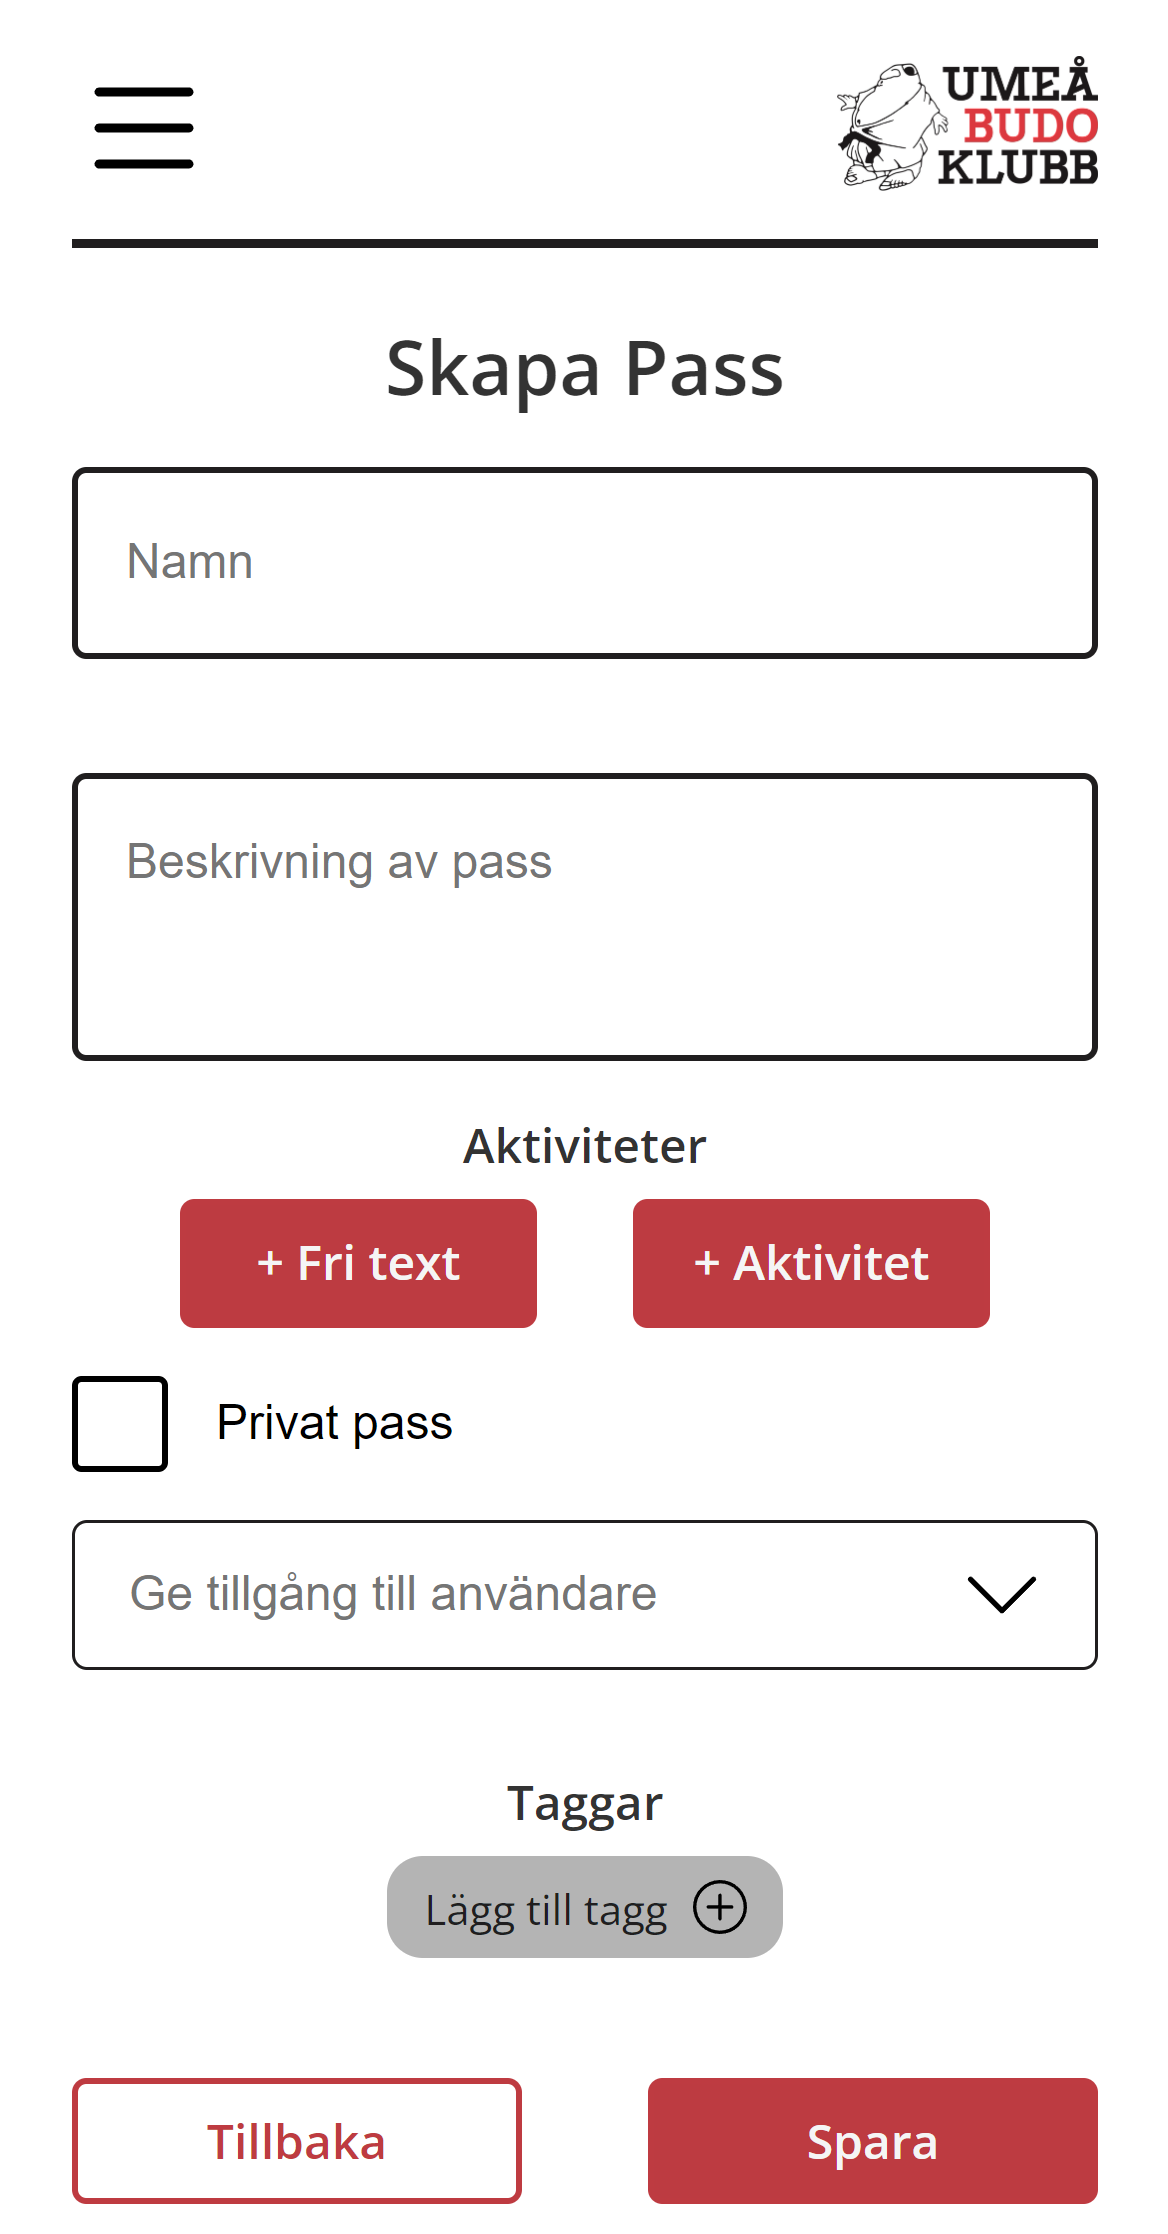
\includegraphics[width=0.9\linewidth]{images/Screens/WorkoutCreate.png}}
            \caption{Sidan för att lägga till ett nytt pass.}
            \label{fig:workoutAdd}
        \end{wrapfigure}
        För att lägga till ett pass, trycker du på den runda knappen nere i högra hörnet med plustecknet \img{images/icons ref/RoundButton.png} på sidan för alla pass. På sidan \term{Skapa pass} kan du ge passet namn och beskrivning. Dagens datum kommer automatiskt läggas till som dagen när passet skapades och kan inte redigeras. När du skapar passet kan du även lägga till övningar och tekniker med hjälp av knappen \button{+ Aktivitet}. Det går även att skapa en "fritext"-aktivitet för detta pass med hjälp av knappen \button{+ Fri text}. När du skapar ett pass väljer du om det ska vara privat eller inte, ett privat pass kan endast visas av den som skapat det, admins och andra användare som man gett tillgång till i rutan \textit{"Ge till gång till användare"}. När du ger en annan användare tillgång till passet kan den både redigera och se det i listan för alla pass. Sen väljer du taggar som ska kopplas till passet genom att klicka på \textit{"Lägg till tagg"}. För att spara det nya passet trycker du på knappen \button{Spara}.

    \subsection{Redigera och ta bort pass}
        \begin{wrapfigure}[5]{r}{0.3\textwidth}
            \vspace{-35pt}
            \fcolorbox{secondary}{background}{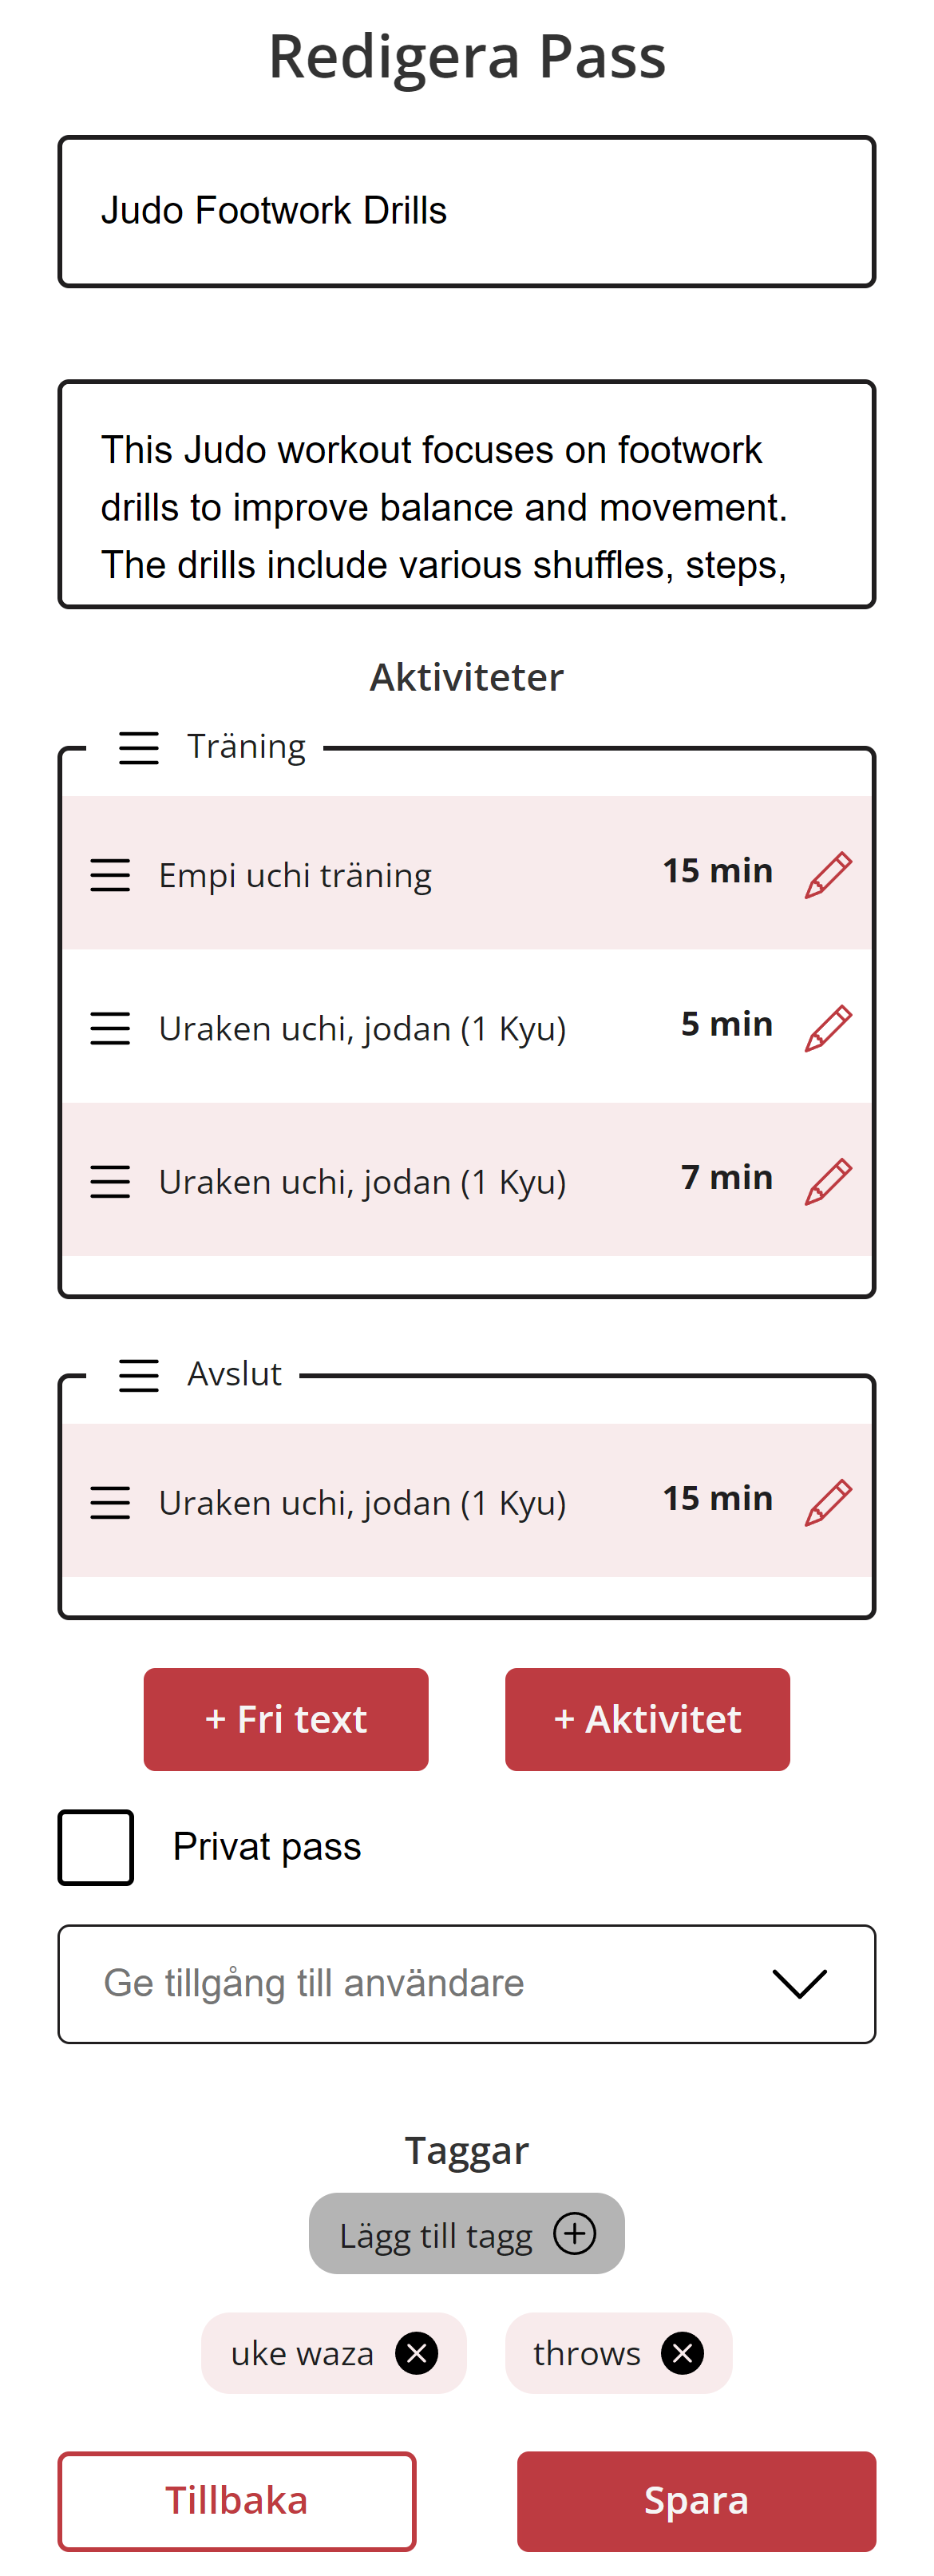
\includegraphics[width=0.9\linewidth]{images/Screens/WorkoutEdit.png}}
            \caption{Sidan för att redigera ett pass.}
            \label{fig:workoutEdit}
        \end{wrapfigure}
        För att redigera eller ta bort ett redan skapat pass går du till passets detaljsida. Klicka sedan på redigeringssymbolen \img{images/icons ref/pencil.png} bredvid passets namn. Där kan du ändra samma detaljer som vid skapandet av ett pass. Om du vill ta bort passet så klicka på ta symbolen \img{images/icons ref/trash.png}. När ett pass försvinner så tas det bort från alla tillfällen som har kopplat det passet.

\newpage
\section{Aktiviteter}
    Med aktiviteter menas både \term{Övningar} och \term{Tekniker}. Genom navigationsmenyn kan du komma till sidan som listar alla övningarna och en annan sida som listar alla tekniker. På dem kan du se, söka efter, ändra, ta bort och lägga till aktiviteter. Det är dock vissa skillnader när det kommer de olika sidorna som beskrivs nedan.

    \subsection{Övningar}
        Övningar används i olika träningspass och kan vara allt ifrån armhävningar och sit-ups till avslappningsmoment och meditation. Dessa sparas med en valfri tid. Du kan även lämna kommentarer på övningen. Sökning på övningar sker med fritext och taggar (valfritt). Övnings-sidan kan även sorteras efter namn eller tid. För att lägga till en övning, tryck på knapp \img{images/icons ref/RoundButton.png}. Du kan ge övningen ett namn, beskrivning, en tid, taggar samt bild ifall så önskas. Om du vill fortsätta skapa övningar kan du klicka i det alternativet, då kommer du att stanna på sidan för att skapa övningar och inte dirigeras vidare vid skapandet av övningen. I så fall finns också ett alternativ att rensa redan ifylld text. För att redigera eller ta bort en övning, klicka på övningens namn. För att redigera, tryck på pennan \img{images/icons ref/pencil.png} bredvid namnet. Där kan du ändra samma detaljer som vid skapandet av en övning. För att ta bort övningen, tryck på soptunnan \img{images/icons ref/trash.png} bredvid redigeringssymbolen. När en övning tas bort försinner den från alla pass den ingår i.
    \begin{figure}[h!]
    \centering
        \fcolorbox{secondary}{background}{
        \centering
            \begin{subfigure}[b]{0.3\textwidth}
                 \centering
                 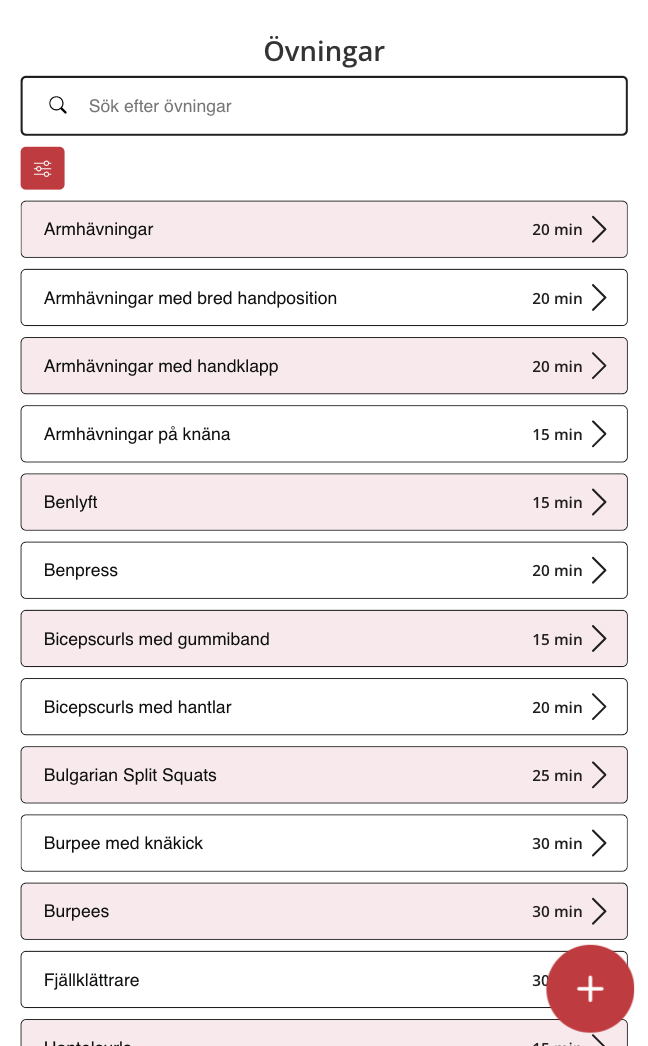
\includegraphics[width=\textwidth]{images/Screens/Exercise.png}
                 \caption{Sidan för alla övningar.}
                 \label{fig:exercise}
            \end{subfigure}
            \hfill
            \begin{subfigure}[b]{0.3\textwidth}
                 \centering
                 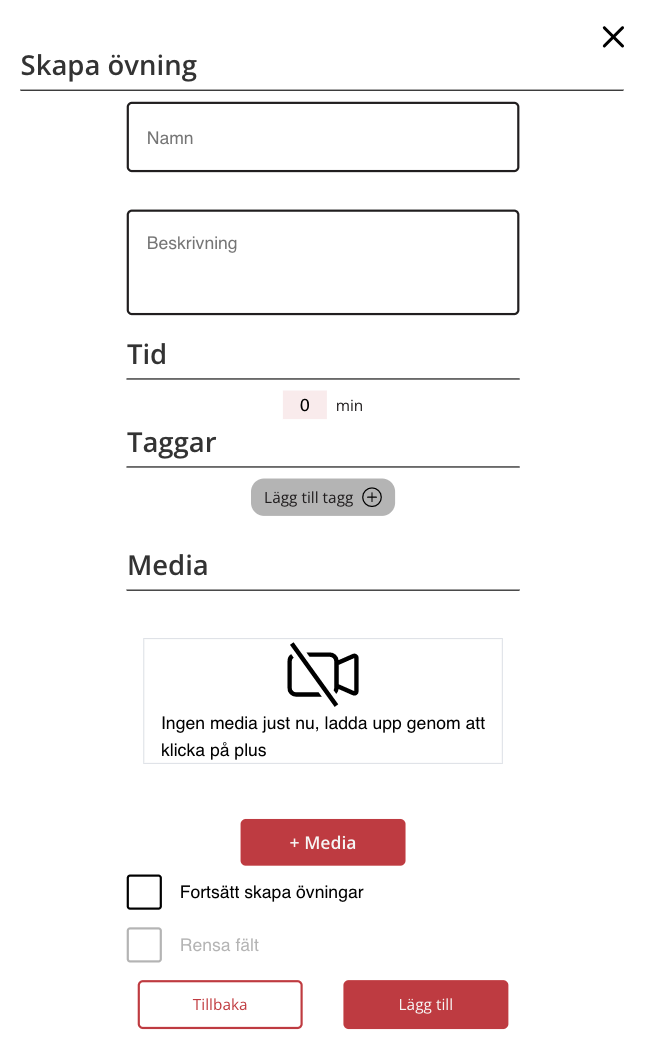
\includegraphics[width=\textwidth]{images/Screens/ExerciseCreate.png}
                 \caption{Sidan för att skapa en ny övning.}
                 \label{fig:exerciseCreate}
            \end{subfigure}
            \hfill
            \begin{subfigure}[b]{0.3\textwidth}
                 \centering
                 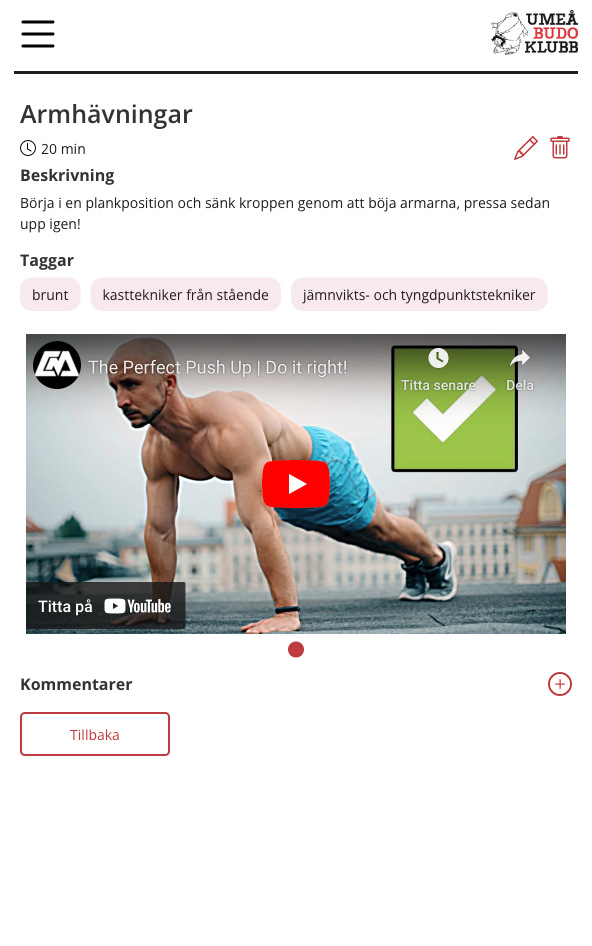
\includegraphics[width=\textwidth]{images/Screens/ExerciseDetail.png}
                 \caption{Detaljsidan för en övning.}
                 \label{fig:exerciseDetail}
            \end{subfigure}
            }
        \caption{De sidor som relaterar till \term{Övningar}.}
        \label{fig:exerciseFig}
    \end{figure}

    \newpage
    \subsection{Tekniker}
        Teknikerna är tekniker som används inom Budo. De är moment och rörelser som ofta är bundna till en viss bältesgrad.
        Sökning på tekniker sker med fritext och taggar (valfritt). Här kan man också filtrera resultaten på bälten, samt Kihon (grundtekniker).
        För att lägga till en teknik, tryck på plusknappen \img{images/icons ref/RoundButton.png}. Du kan ge tekniken ett namn, beskrivning, om den är Kihon eller inte, bälten kopplade till tekniken, taggar samt bild ifall så önskas. För att lägga till den nya tekniken trycker du på knappen \button{Lägg till}. Om du vill fortsätta skapa tekniker kan du klicka i det alternativet, då kommer du att stanna på sidan för att skapa tekniker och inte dirigeras vidare vid skapandet av tekniken. I så fall finns också ett alternativ att rensa redan ifylld text. För att redigera eller ta bort en teknik, klicka på teknikens namn. För att redigera, tryck på redigeringssymbolen \img{images/icons ref/pencil.png} bredvid namnet. Där kan du ändra samma detaljer som vid skapandet av en teknik. För att ta bort tekniken, tryck på soptunnan \img{images/icons ref/trash.png} bredvid redigeringssymbolen. När en teknik tas bort försvinner den från alla pass den ingår i.
        \begin{figure}[h]
        \centering
            \fcolorbox{secondary}{background}{
            \centering
                \begin{subfigure}[b]{0.25\textwidth}
                     \centering
                     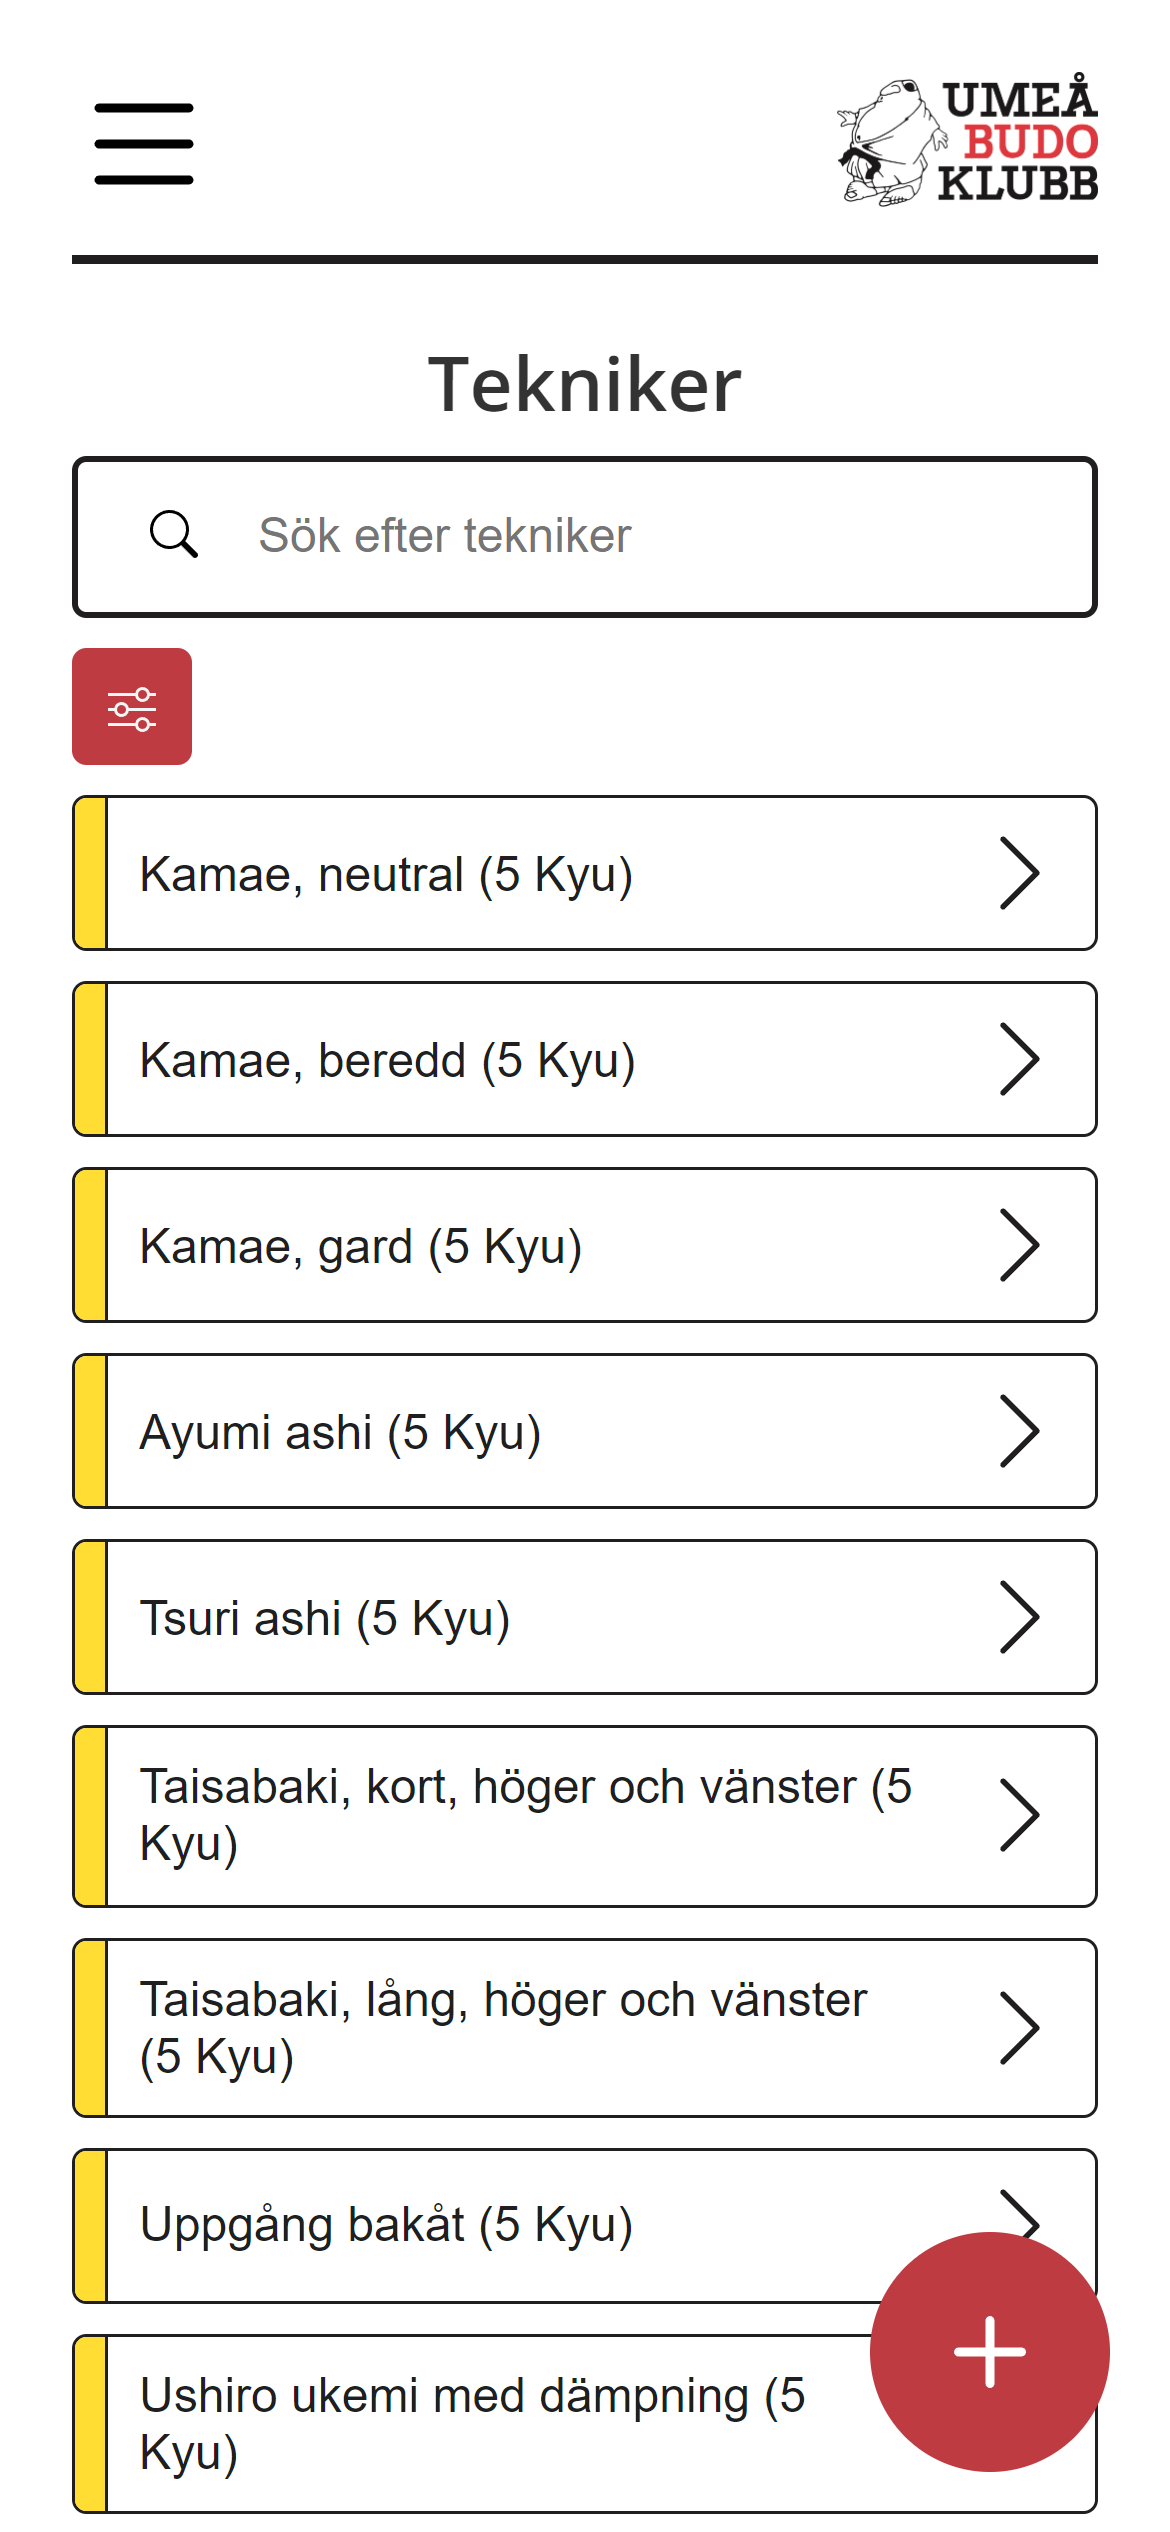
\includegraphics[width=\textwidth]{images/Screens/Technique.png}
                     \caption{Sidan för alla tekniker.}
                     \label{fig:technique}
                \end{subfigure}
                \hfill
                \begin{subfigure}[b]{0.25\textwidth}
                     \centering
                     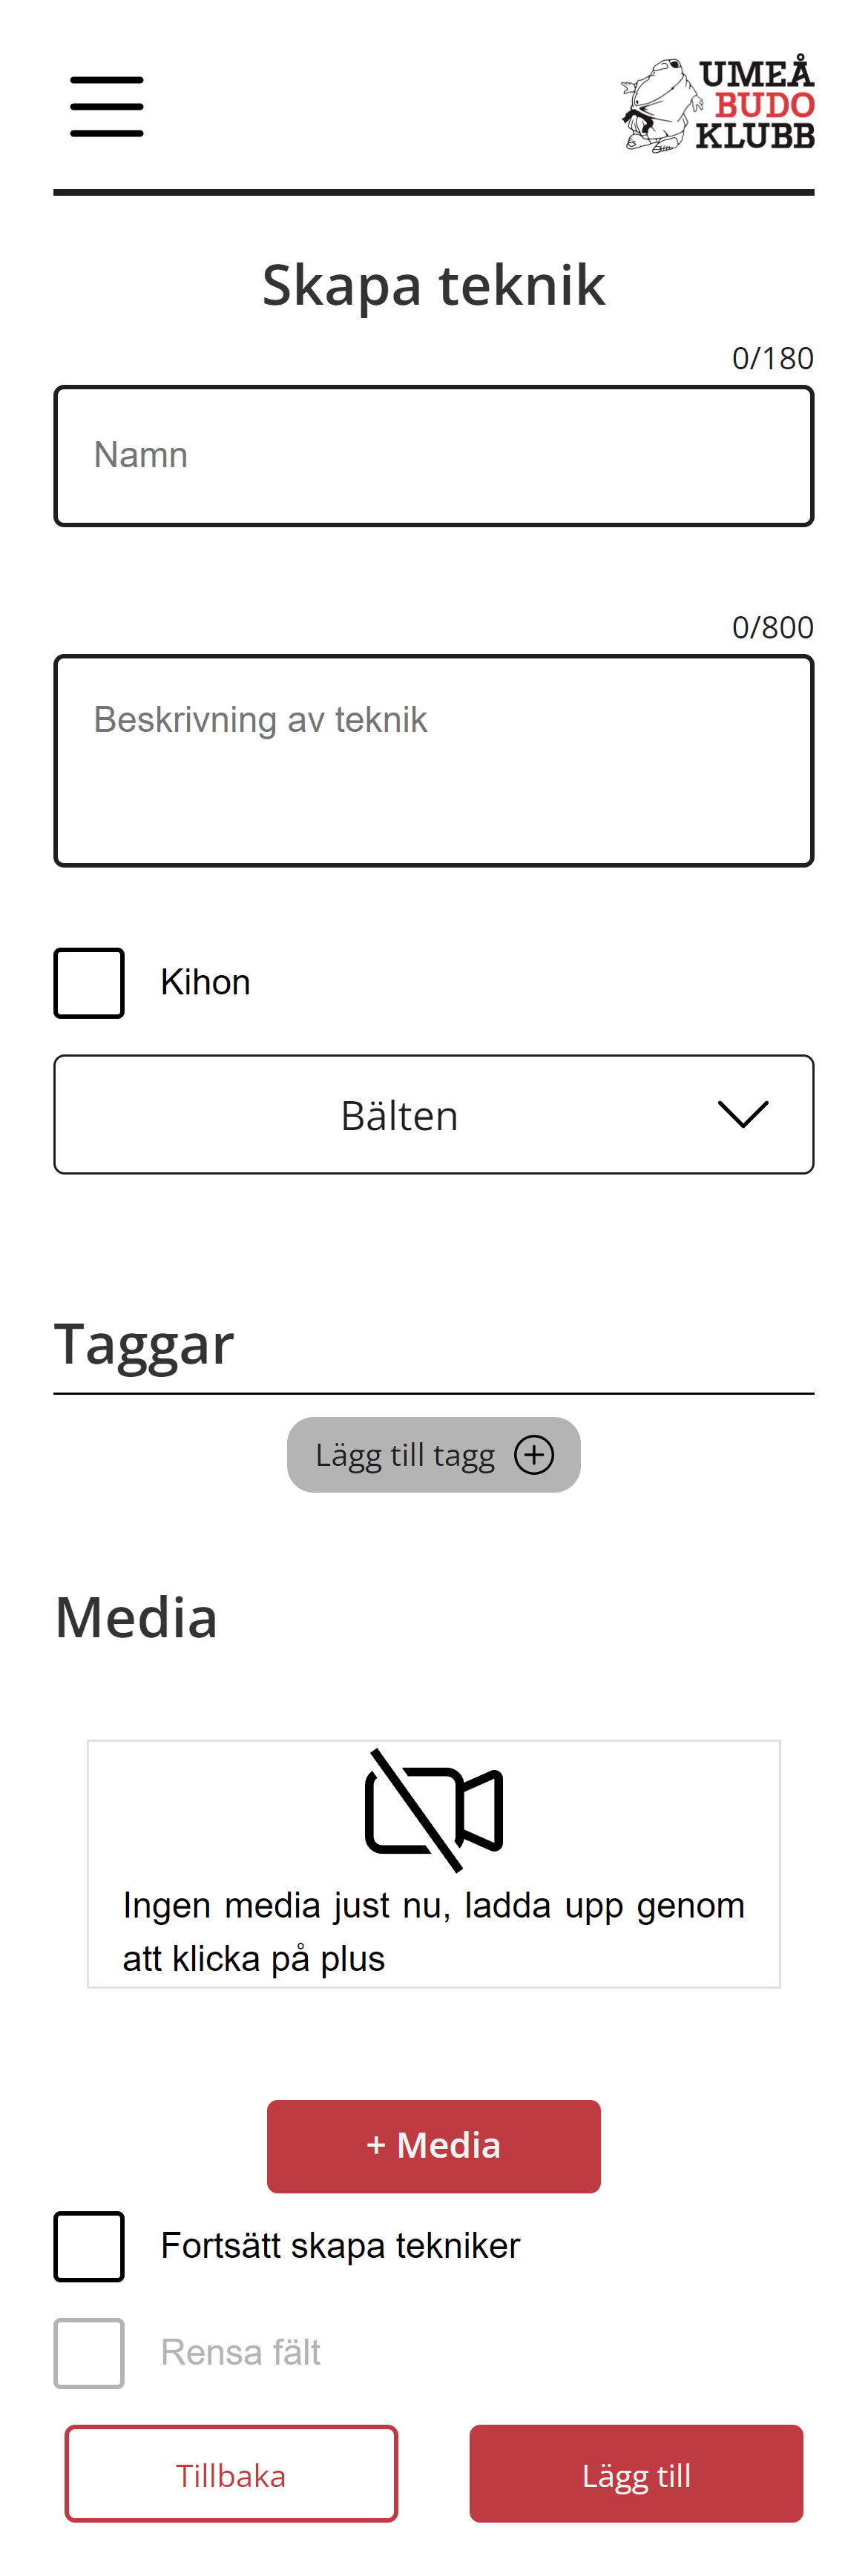
\includegraphics[width=\textwidth]{images/Screens/TechniqueCreate.png}
                     \caption{Sidan för att skapa en teknik.}
                     \label{fig:techniqueCreate}
                \end{subfigure}
                \hfill
                \begin{subfigure}[b]{0.25\textwidth}
                     \centering
                     \includegraphics[width=\textwidth]{images/Screens/TechniqueDetail.png}
                     \caption{Detaljsidan för en teknik.}
                     \label{fig:techniqueDetail}
                \end{subfigure}
                }
            \caption{De olika sidorna som relaterar till \term{Tekniker}.}
            \label{fig:techniquesFig}
        \end{figure}
\newpage
\section{Användarroller}
    På hemsidan existerar det tre olika roller med olika behörigheter som påverkar hur man kan se och redigera innehållet på sidan. När en ny användare skapas väljer men en av de tre roller direkt. Om man vill ändra en användares roll måste en admin göra det via admin-sidan.

    \subsection{Admin}
        \begin{wrapfigure}[20]{r}{0.3\textwidth}
            \vspace{-15pt}
            \fcolorbox{secondary}{background}{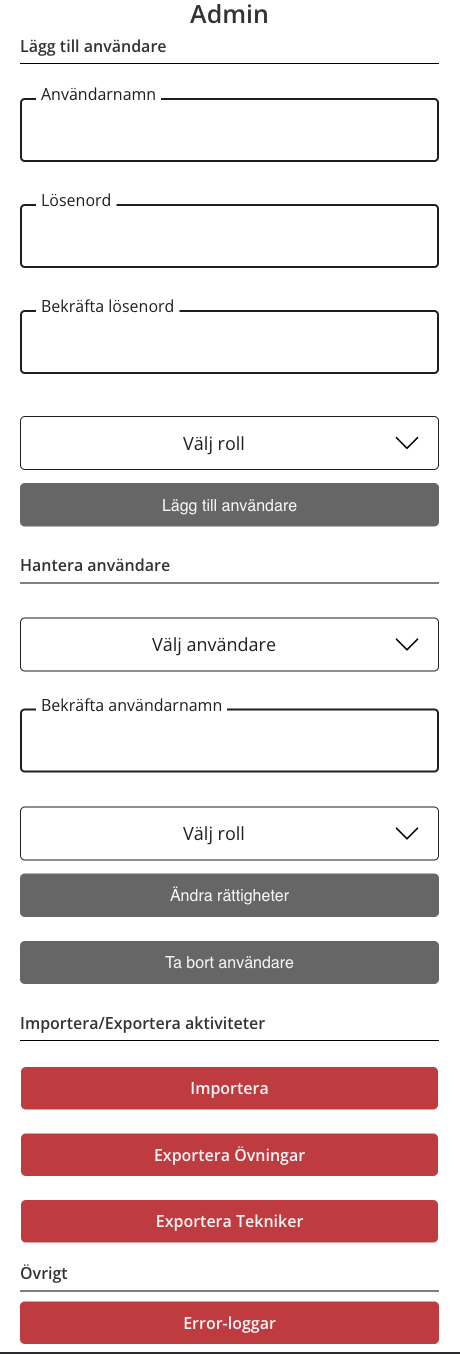
\includegraphics[width=0.9\linewidth]{images/Screens/Admin.png}}
            \caption{Adminsidan som endast visas för admins.}
            \label{fig:admin}
        \end{wrapfigure}
        Som admin kan du skapa, redigera och ta bort alla grupper, tillfällen, pass, övningar samt tekniker. Du kan skapa nya användare för inloggning och hantera de redan existerande användarna. Du kan importera och exportera övningar och tekniker. Import till databasen sker endast i tillägg. Importering misslyckas om JSON filen innehåller en teknik eller övning med ett namn som redan finns i databasen, eller om något fält är tomt. Filerna som importeras ska vara JSON-filer med samma format som det som ges vid export. Som admin har du även tillgång till error-loggar. Du kan utföra de mesta administrativa arbetet via sidan \term{Admin}. Den når du genom navigationsmenyn på alla sidor efter att du loggat in. Det måste alltid finnas en admin, därför kommer du ej kunna ta bort en admin om den är den sista som är kvar.

    \subsection{Utökad användare}
        Som utökad användare kan du skapa grupper, tillfällen, pass och övningar. Du kan redigera och ta bort alla grupper, tillfällen och övningar även de som någon annan skapat. Du kan redigera och ta bort de pass som du själv har skapat. Du kan varken skapa, redigera eller ta bort tekniker.

    \subsection{Användare}
        Som användare kan du skapa grupper, tillfällen och pass samt redigera och ta bort det innehåll som du själv äger eller är medlem på. Du kan varken skapa, redigera eller ta bort tekniker eller övningar.

\newpage
\section{Min sida}
    På \term{Min Sida} kan du se information angående din användare. På den första fliken \button{Favoritpass} ser du de pass som du har favoriserat. På den andra fliken \button{Mina Pass} hittar du de pass som du har skapat. På båda pass-flikarna kan du även favorisera och av-favorisera pass samt navigera till passets detaljsida genom att trycka på passet. På den sista fliken \button{Inställningar} kan du ändra inställningar för din användare. Du kan ändra ditt lösenord samt användarnamn.

    \vspace{15pt}
    \begin{figure}[h]
        \fcolorbox{secondary}{background}{
        \centering
             \begin{subfigure}[b]{0.3\textwidth}
                 \centering
                 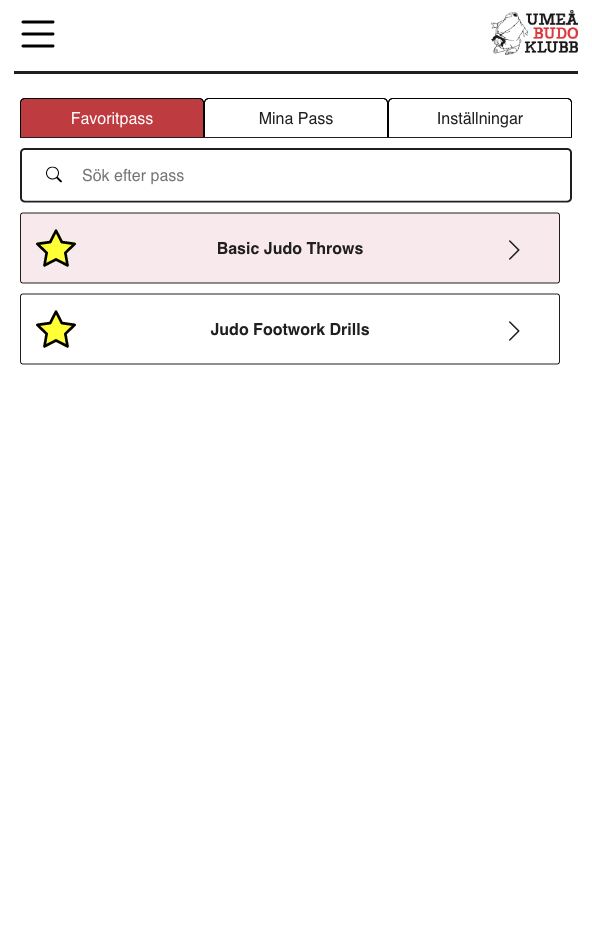
\includegraphics[width=\textwidth]{images/Screens/UserFavorites.png}
                 \caption{Favoritpass-fliken}
                 \label{fig:userFavorites}
             \end{subfigure}
             \hfill
             \begin{subfigure}[b]{0.3\textwidth}
                 \centering
                 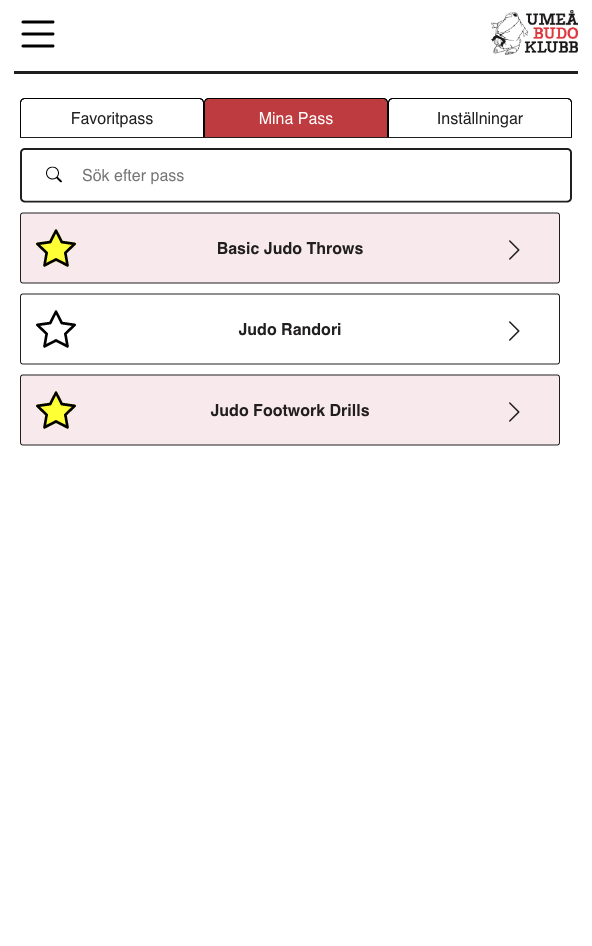
\includegraphics[width=\textwidth]{images/Screens/UserWorkouts.png}
                 \caption{Dina pass-fliken}
                 \label{fig:userWorkouts}
             \end{subfigure}
             \hfill
             \begin{subfigure}[b]{0.3\textwidth}
                 \centering
                 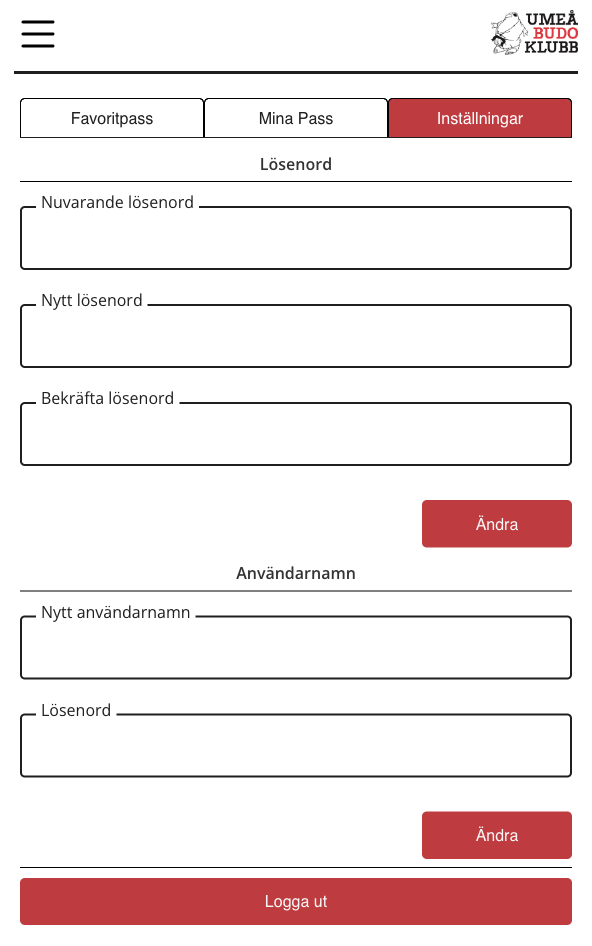
\includegraphics[width=\textwidth]{images/Screens/UserSettings.png}
                 \caption{Inställningar-fliken}
                 \label{fig:userSettings}
             \end{subfigure}
             }
        \caption{De tre flikarna som finns på \term{Min sida}.}
        \label{fig:userFig}
    \end{figure}

}
\end{document}
